% !TeX root = ../tfg.tex
% !TeX encoding = utf8

\chapter{Introducción}
\label{cap:capitulo1}
\section{Contexto}
La inteligencia artificial es la disciplina mediante la cual se diseñan algoritmos mediante los cuales se permite a las máquinas asimilar comportamientos humanos. En 1950 el matemático Alan Turing formuló la siguiente pregunta: "¿Pueden pensar las máquinas?". Publicó su artículo llamado 'Computing Machinery and Intelligence', presentando el famoso test de Turing, por el cual se permitía evaluar si el comportamiento de una máquina es o no indistinguible al de un ser humano. Si bien el interés en este tipo de cuestiones ya existía en la época de la Antigua Grecia, a partir de esta pregunta se generó un creciente interés en el tema, llegando a abrir una gran cantidad de líneas de investigación al respecto. Consecuencia de esto, se ha llegado a la creación de inteligencias artificiales de fuerte impacto como el conocido ChatGPT. Sin embargo, estos algoritmos no están exentos de los clásicos ataques informáticos para hacerlos fallar, por lo que es natural preguntarse sobre maneras para prevenir estos ataques, e incluso crearlos para descubrir más vulnerabilidades de los mismos.

Una de las disciplinas de la inteligencia artificial es el aprendizaje automático, en el que se puede distinguir ramificaciones del mismo, como el aprendizaje supervisado, el aprendizaje por refuerzo, el aprendizaje no supervisado,... Mención especial merece el aprendizaje profundo, o deep learning, que es una de las ramificaciones del aprendizaje automático, con creciente interés actualmente, y sobre el que se va a desarrollar el presente trabajo.

En primer lugar, se presentarán una serie de resultados auxiliares para poder construir matemáticamente qué es una red neuronal profunda (multicapa), que es el algoritmo clave en el aprendizaje profundo, y la justificación de varios algoritmos derivados del concepto de red neuronal. Acto seguido, se darán dos formas de clasificación de los ataques que pueden sufrir una red, dando a entender que ningún algoritmo es completamente seguro.

Los siguientes apartados tratarán de justificar la existencia tanto de los ataques causativos como de los ataques exploratorios, atacando al modelo usando tanto las debilidades existentes en el mismo como las de los datos de entrenamiento. Además, se mencionarán y desarrollarán brevemente otros puntos de vista que exponen investigadores del campo, apoyándose en resultados de topología algebraica o teoría de juegos. Finalmente, se podrá intuir que no existe una propiedad universal que sea la culpable de la existencia de los ataques, teniendo que mejorar la robustez de los modelos de manera independiente entre las características del mismo.

%, y sobre el que se desarrollará este trabajo, apoyado por resultados matemáticos consistentes.

\newpage

\section{Resultados auxiliares}

Para poder desarrollar correctamente todos los resultados sobre los que trata este trabajo, es necesario hacer uso de teoremas, definiciones y otras proposiciones (un ejemplo de ello es el poder demostrar el teorema de aproximación universal). En este apartado se mencionarán aquellos necesarios para el correcto desarrollo de la memoria, demostrando aquellos que sean más relevantes.

En primer lugar, los conjuntos sobre los que el algoritmo aprende son espacios medibles.

\begin{definicion}[Espacio medible]
Dado un conjunto $X$ y una $\sigma$-álgebra $\mathbb{B}$ en $X$, un espacio medible es ($X,\mathbb{B}$), donde una $\sigma$-álgebra sobre $X$ es una familia $B \subset \mathbb{P}(X)$ (partes de $X$) no vacía de subconjuntos tal que se cumple:
\begin{itemize}
	\item $X \in \mathbb{B}$.
	\item Si $B\in\mathbb{B} $ entonces su complementario $X-B \in \mathbb{B}$.
	\item Si se tiene un conjunto numerable de subconjuntos de $\mathbb{B}$ entonces su unión también está en $\mathbb{B}$.
\end{itemize}
Además, si se le consigue asociar una medida $\mu$, se denotará al espacio como la terna ($X,\mathbb{B},\mu$) (los espacios medibles no necesitan tener asociada una medida).
\end{definicion}

Por otro lado, también se hará uso de los espacios normados (de funciones integrables en el sentido de Lebesgue). Conviene definir espacio vectorial y de ahí desprender la definición de espacio normado (ambas definiciones fundamentales para el apoyo en algunos resultados).

\begin{definicion}[Espacio vectorial]
Un espacio vectorial es una terna ($V,+,\cdot$) donde $V$ es no vacío, $+:V\times V \to \mathbb{K}$ es la operación suma y $\cdot:\mathbb{K}\times V \to V$ es el producto escalar, y cumple las siguientes propiedades, con $u,v,w \in V \text{ y } \lambda,\mu \in \mathbb{K}$:
\begin{itemize}
	\item $u+(v+w)=(u+v)+w$ (asociativa).
	\item $u+v=v+u$ (conmutativa).
	\item $\exists e\in V \text{ tal que } e+v=v+e=v$ (elemento neutro).
	\item $\forall v\in V \text{ } \exists w \text{ tal que } v+w=w+v=e$ (elemento opuesto).
	\item $\lambda(\mu v)=(\lambda\mu)v$ (pseudo-asociativa).
	 \item $\lambda(u+v)=\lambda u+\lambda v$ y $(\lambda+\mu)v=\lambda v+\mu v$ (distributiva).
	\item $\mathbb{1}v=v$ (unimodular).
\end{itemize}

$\mathbb{K}$ es un cuerpo, y generalmente se tomará $\mathbb{K}=\mathbb{R}$.
\end{definicion}

\begin{definicion}[Espacio normado]
Sea $V$ un espacio vectorial sobre $\mathbb{K}$. Se dirá que $V$ es un espacio normado si tiene asignado una norma, esto es, una aplicación

$$||\cdot||: V \to \mathbb{R}$$
$$x \to ||x||$$

que cumple

\begin{itemize}
    \item $||x|| \geq 0 \text{ } \forall x \in V$ y $||x||=0$ si, y solo si, $x=0$ (No negatividad).
    \item $||\lambda x||=|\lambda|\cdot ||x|| \text{ } \forall x \in V, \forall \lambda \in \mathbb{K}$ (Homogeneidad).
    \item $||x+y|| \leq ||x|| + ||y|| \text{ } \forall x,y \in V$ (Desigualdad triangular).
\end{itemize}
\end{definicion}

Aunque espacios normados hay bastantes, tando de dimensión finita como infinita, se hará uso de un tipo de espacio normado de dimensión infinita: los espacios $L_p$.

\begin{definicion}[Espacios $L_p$]
Considérese el espacio de todas las funciones integrables en el sentido de Lebesgue, que es un espacio medible. Para $p\in[1,\infty)$ se define el espacio $L^p$ como el espacio de funciones integrables en el sentido de Lebesgue tales que, si $\Omega$ es el dominio de $f$, cumple $\int_{\Omega} |f|^p dx < \infty$. Entonces, su norma se define de la misma manera. Por otro lado, si $p=\infty$, entonces $L^{\infty}$ es el espacio de funciones integrables en el sentido de Lebesgue tales que $\sup\{|f(x)|:x\in\Omega\}<\infty$.
\end{definicion}

\textbf{Aclaración}: Definido $L_p$ para $p\geq 1$, se especifica que si se escribe $L_{loc}^{p}$, entonces la propiedad definida es cierta de forma local (no necesariamente en todo el dominio).

%\begin{teorema}[Teorema de isomorfía (geo I)]
%\end{teorema}

%\begin{proposicion} [Regla de la cadena]
%\end{proposicion}

\begin{teorema}[Teorema de Hahn-Banach]
Sea $V$ un espacio vectorial real, y sea $p: V \to \mathbb{R}$ una función que cumple $p(x+y)\leq p(x)+p(y)$ para todos $x, y \in V$ y $p(\lambda x)=\lambda p(x)$ para $x \in V$ y $\lambda > 0$. Sea $f: M \to \mathbb{R}$ lineal con $M$ subespacio vectorial de $V$ tal que $f(x) \leq p(x)$ para $x \in M$. Entonces existe una aplicación lineal $g: V \to \mathbb{R}$ tal que $g|_{M} = f$ y $g(x) \leq p(x)$ para $x \in V$.
\end{teorema}


A continuación se enuncia un teorema necesario para la prueba del teorema de aproximación universal sobre compactos para redes neuronales, apoyado en conceptos fundamentales en topología como los espacios Hausdorff o los espacios localmente compactos.

\begin{teorema}[Teorema de representación de Riesz-Markov-Kakutani]
Sea $X$ un espacio Hausdorff localmente compacto (todo punto admite una base de entornos compactos, y existen entornos disjuntos para todo par de puntos) y $F$ un funcional lineal positivo en el soporte de las funciones continuas en $X$. Entonces existe una $\sigma$-álgebra $\mathbb{B}$ en $X$ y una única medida $\mu$ en $X$ tal que 

$$F(f)=\int_{X} f(x)d\mu(x) \text{ para todo } f \in C_c(X)$$ 
y cumplen las siguientes propiedades:
\begin{itemize}
	\item $\mu(K)<\infty$ para cada compacto $K \subset X$ ($\mu$ es un medidad $\sigma$-finita).
	\item $\mu(E)=\inf\{\mu(U):E\subset U, U\text{ abierto}\}$ para cada conjunto de Borel $E \in \Sigma$ (regularidad exterior).
	\item $\mu(E) = \sup\{\mu(K) : K \subset E, K \text{ compacto}\}$ para todo $E$ abierto o $E$ conjunto de Borel con $\mu(E) < \infty$ (regularidad interior).
	\item ($X$,$\Sigma$,$\mu$) es un espacio medible completo (toda sucesión de Cauchy es convergente).
\end{itemize}
\end{teorema}

Finalmente se muestran ciertos conceptos y resultados de teoría de la probabilidad necesarios para ciertas demostraciones y presentaciones de resultados de los algoritmos de aprendizaje profundo, tanto en sus fundamentos como en los temas en que se centra este trabajo.

\begin{definicion}[Dominancia estocástica de primer orden]
Sean las variables aleatorias \(X\) e \(Y\) con respectivas funciones de distribución \(F\) y \(G\). Se dirá que \(X\) domina estocásticamente en primer orden a \(Y\) si, y solo si, \(G(x) \leq F(x)\) para todo \(x\) en el dominio.
\end{definicion}

\begin{definicion}[Dominancia estocástica de segundo orden]
Sean $X$ e $Y$ las mismas variables aleatorias. Se dirá que $x$ domina estocásticamente en segundo orden a $Y$ si, y solo si, 
\[\int_{-\infty}^{x} G(t) - F(t) \, dt \geq 0 \quad \forall x \in \mathbb{R}\]
\end{definicion}

\begin{proposicion}[Desigualdad de Markov]
Sea \(X\) una variable aleatoria no negativa tal que \(\exists \mathbb{E}[X]\). Para \(a > 0\), entonces

\[
\mathbb{P}[X \geq a] \leq \frac{\mathbb{E}[X]}{a}
\]

\end{proposicion}

\begin{proof}
Considérese $A$ un suceso, y sea $I_A$ una variable aleatoria que vale 1 si ocurre $A$ y 0 si no ocurre. Entonces

$$aI_{(|X|\geq a)}\leq|X|$$

Así,

$$\mathbb{E}[aI_{(|X|\geq a)}]\leq \mathbb{E}[|X|]$$

Por linealidad, y tal y como se define $I$ es cierto que $a\mathbb{E}[I_{(|X|\geq a)}]=a \mathbb{P}[|X| \geq a] $, por lo que se obtiene
$$a\mathbb{P}[|X| \geq a] \leq \mathbb{E}[|X|]$$ 
de donde, como $a>0$, se desprende la desigualdad buscada.

\end{proof}

Por último, para ciertas demostraciones que se harán más adelante, es necesario hacer uso de las cotas de Chernoff. Dichas cotas de una variable aleatoria $X=\sum_{i=1}^n X_i$, suma de variables aleatorias independientes, se obtienen al aplicar $e^{tX}$ para cierto $t$.

Comenzando por la desigualdad de Markov, usando la independencia, se obtiene

$$\mathbb{P}[X \geq a] = \mathbb{P}[e^{tX} \geq e^{ta}] \leq \frac{\mathbb{E}[e^{tX}]}{e^{ta}} = e^{-ta} \mathbb{E} \left[ \prod_{i=1}^n e^{tX_i} \right]$$

Resolviendo una optimización sobre $t$ y de nuevo usando la hipótesis de independencia,

\begin{equation} \label{optimiza}
\mathbb{P}[X \geq a] \leq \min_{t>0} e^{-ta} \prod_{i=1}^n \mathbb{E}[e^{tX_i}]
\end{equation}

De manera análoga,

$$\mathbb{P}[X \leq a] = \mathbb{P}[e^{-tX} \geq e^{-ta}]$$

y

$$\mathbb{P}[X \leq a] \leq \min_{t>0} e^{ta} \prod_{i=1}^n \mathbb{E}[e^{-tX_i}]$$

Esto se puede formalizar de forma más precisa, dando varias posibles cotas para distintas situaciones. En primer lugar, se tiene el siguiente teorema:

\begin{teorema}[Teorema para la forma aditiva o de Chernoff-Hoeffding]

Sean $X_1,...,X_n$ variables aleatorias independientes e idénticamente distribuidas en $\{0,1\}$. Sea $p = \mathbb{E}[X_1]$ y $\epsilon>0$. Supóngase que se cumple

$$\mathbb{P} \left[ \frac{1}{n} \sum_{i=1}^n X_i \geq p+\epsilon \right] \leq \left( \left( \frac{p}{p+\epsilon} \right)^{p+\epsilon} \left( \frac{1-p}{1-p-\epsilon} \right)^{1-p-\epsilon} \right)^n = e^{-D(p+\epsilon\|p)n}$$

$$\mathbb{P} \left[ \frac{1}{n} \sum_{i=1}^n X_i \leq p-\epsilon \right] \leq \left( \left( \frac{p}{p-\epsilon} \right)^{p-\epsilon} \left( \frac{1-p}{1-p+\epsilon} \right)^{1-p+\epsilon} \right)^n = e^{-D(p-\epsilon \| p)n}$$

con 

$$D(x \| y)=x ln(\frac{x}{y}) + (1-x)ln \left( \frac{1-x}{1-y} \right)$$

la llamada \textit{divergencia Kullback-Leibler} entre dos variables aleatorias dque forman una distribución de Bernoulli con parámetros $x$ e $y$.

Si $p\geq \frac{1}{2}$ entonces

$$\mathbb{P} \left[ X > np+x \right] \leq \exp \left( - \frac{x^2}{2np(1-p)} \right)$$

\end{teorema}

\begin{proof}
Sean $q=p+\epsilon$ y $a=nq$. Usando $a$ en la ecuación obtenida de la optimización sobre $t$, \ref{optimiza}, se consigue

$$\mathbb{P} \left[ \frac{1}{n} \sum_{i=1}^n X_i \geq q \right] \leq \inf_{t>0} \frac{\mathbb{E}[\prod_{i=1}^n e^{tX_i}]}{e^{tnq}} = \inf_{t>0} \left( \frac{\mathbb{E}[e^{tX_i}]}{e^{tq}} \right)^n$$

Dado que $\mathbb{P}[X_i=1]=p$ y $\mathbb{P}[X_i=0]=1-p$, entonces

$$\left( \frac{\mathbb{E}[e^{tX_i}]}{e^{tq}} \right)^n = \left( \frac{pe^{t} + (1-p)}{e^{tq}} \right)^n = \left( pe^{(1-q)t} + (1-p) e^{-qt} \right)^n$$

Por lo que usando

$$\frac{d}{dt} \left( pe^{(1-q)t} + (1-p)e^{-qt} \right) = (1-q)pe^{(1-q)t} - q(1-p)e^{-qt} = 0$$

podemos obtener el ínfimo, que es

$$(1-q)pe^{(1-q)t} = q(1-p)e^{-qt}$$
$$(1-q)pe^t = q(1-p)$$

y despejando

$$t = ln \left( \frac{(1-p)q}{(1-q)p} \right)$$

Como $q>p$, entonces $t>0$, por lo que la cota se satisface para $t$. Sustituyendo las ecuaciones anteriores aplicando logaritmos, se llega

\begin{align*}
ln \left( pe^{(1-q)t} + (1-p)e^{-qt} \right) = \\
&=ln \left( e^{-qt} (1-p+pe^t) \right) = \\
&=ln \left( e^{-q ln \left( \frac{(1-p)q}{(1-q)p} \right)} \right) + ln \left( 1-p+pe^{ln \left( \frac{1-p}{1-q} \right)}e^{ln \left( \frac{q}{p} \right)} \right) = \\
&=-q ln \left( \frac{1-p}{1-q} \right) -q ln \left( \frac{q}{p} \right)+ln \left( 1-p+p \left( \frac{1-p}{1-q} \right) \frac{q}{p} \right) = \\
&= -q ln \left( \frac{1-p}{1-q} \right) -q ln \left( \frac{q}{p} \right) + ln \left(  \frac{(1-p)(1-q)}{1-q} + \frac{(1-p)q}{1-q} \right) = \\
&= -q ln \left( \frac{q}{p} \right) + \left( -q ln \left( \frac{1-p}{1-q} \right) + ln \left( \frac{1-p}{1-q} \right) \right) = \\
&= -q ln \left( \frac{q}{p} \right) + (1-q) ln \left( \frac{1-p}{1-q} \right) = \\
&= -D(q \| p)
\end{align*}

Obteniendo al final $\mathbb{P} \left[ \frac{1}{n} \sum_{i=1}^n X_i \geq p+\epsilon \right] \leq e^{-D (p+\epsilon  \| p)n}$

El otro caso se prueba de manera similar definiendo, para cada $i$, la variable aleatoria $Y_i = 1-X_i$.

\end{proof}

Sin embargo, se pueden obtener cotas más simples relajando las hipótesis del teorema, usando $D(p+x \| p) \geq 2x^2$ por ser $D(p+x \| p)$ convexo y cumplirse

$$\frac{d^2}{dx^2} D(p+x \| p) = \frac{1}{(p+x)(1-p-x)} \geq 4= \frac{d^2}{dx^2} (2x^2)$$ 

\begin{teorema}[Teorema para la forma multiplicativa de las cotas de Chernoff o de Chernoff multiplicativa]
Sean $X_1,...X_n$ variables aleatorias independientes en $\{0,1\}$ y $X = \sum_{i=1}^n X_i$, con $S = \mathbb{E}[X]$ la suma de valores esperados. Entonces para todo $\delta > 0$,

$$\mathbb{P} \left[ X > (1+\delta) S \right] < \left( \frac{e^\delta}{(1+\delta)^{1+\delta}} \right)^S$$
\end{teorema}

\begin{proof}
Si $p_i = \mathbb{P}[X_i=1]$, usando \ref{optimiza},

\[
\mathbb{P}[X > (1+\delta) S] \leq \inf_{t>0} \frac{\mathbb{E}\left[\prod_{i=1}^n \exp(tX_i)\right]}{\exp(t(1+\delta)S)} = \inf_{t>0} \frac{\prod_{i=1}^n \mathbb{E}[e^{tX_i}]}{\exp(t(1+\delta)S)} = \inf_{t>0} \frac{\prod_{i=1}^n (p_i e^t + (1-p_i))}{\exp(t(1+\delta)S)}
\]


Reescribiendo $p_i e^t + (1-p_i)$ como $p_i (e^t - 1)+1$ y viendo que $1+x \leq e^x$, se obtiene $x=p_i(e^t-1)$. Por lo tanto

$$\mathbb{P}[X > (1+\delta)S] < \frac{\prod_{i=1}^n \exp(p_i (e^t-1))}{\exp(t(1+\delta)S)} =  \frac{\exp((e^t-1) \sum_{i=1}^n p_i)}{\exp(t(1+\delta)S)} = \frac{\exp((e^t-1)S)}{\exp(t(1+\delta)S)}$$

Si se escribe $t=ln (1+\delta)$ de tal forma que $t>0$ para $\delta > 0$, se puede sustituir y

$$\frac{\exp((e^t-1) S)}{\exp(t(1+\delta)S)} = \frac{\exp((1+\delta-1)S)}{(1+\delta)^{(1+\delta)S}} = \left[ \frac{e^\delta}{(1+\delta)^{1+\delta}} \right]^S$$

\end{proof}

\newpage

\section{Deep Learning: Fundamentos}

Los algoritmos de aprendizaje profundo intentan simular al cerebro humano en su forma de trabajar. A partir de una serie de elementos llamados neuronas, se conectan entre ellas para llevar a cabo la realización de tareas como clasificación.

Este es un algoritmo que, basado en ciertos datos, aprende e intenta generalizar a partir de ellos. Es necesario preguntarse qué implica aprender para un algoritmo. Sean $\mathcal{X}$, $\mathcal{Y}$ y $\mathcal{Z}$ tres espacios medibles, donde $\mathcal{Z}$ es el espacio de las posibles entradas a un algoritmo, y $\mathcal{M(X,Y)}$ cierto espacio de pares (entrada-salida). Denótese como $\mathcal{L}$ a la función coste, $\mathcal{L}: \mathcal{M(X,Y)} \times \mathcal{Z} \to \mathbb{R}$. 

El objetivo de que un algoritmo aprenda se conseguirá si se obtiene cierto subconjunto $\mathcal{F} \subset \mathcal{M(X,Y)}$, llamado subconjunto de hipótesis, y cierto algoritmo de aprendizaje $\mathcal{A}: \bigcup_{n \in \mathbb{N}} \mathcal{Z}^n
 \to \mathcal{F}$ tal que si se escribe a los datos para el aprendizaje como $s = (z^{(i)})_{i=1}^{n} \in \mathcal{Z}^n$ con $n \in \mathbb{N}$ pueda encontrar un modelo $f_s = \mathcal{A}(s) \in \mathcal{F}$ que pueda tanto predecir bien los datos del subconjunto de hipótesis como generalizar correctamente para cualquier entrada de elementos de cierto $\mathcal{B} \subset \mathcal{M(X,Y)}$ con $\mathcal{B} \cap \mathcal{F} = \emptyset$.
 
En general, en el momento del entrenamiento de un algoritmo, se hace uso de la función coste cuadrática (se supone que se trabaja con datos cuantitativos y un modelo que predice valores reales), que se busca minimizar. Es decir, si $$\mathcal{L}(f,(x,y)) = (f(x)-y)^2$$  se busca que tienda a 0 para la predicción. En este caso $(x,y)$ es un par (entrada,salida) y $f(x)$ es la predicción hecha. De ahí se desprende que tenga sentido hacer la diferencia entre ellos. Por último, el cuadrado evita que tome valores negativos, y como la función $g(x)=x^2$ es simétrica respecto al eje $Y$, y es monótona tanto a izquierda como derecha de su vértice, no se perderá información en ninguna evaluación.
Caso aparte es si el problema es de clasificación binaria, donde se toma $$\mathcal{L}(f,(x,y)) = \mathbb{1}_{(-\infty,0)}(y \cdot f(x)) = \begin{cases}
    1, & \text{si } y \cdot f(x) < 0 \\
    0, & \text{en otro caso}
\end{cases}
$$ donde $x \in \mathbb{R^d}$ para cierto $d \in \mathbb{N}$, $y \in \{-1,1\}$.

Finalizado el breve inciso, se comienza a construir rigurosamente una red neuronal, aportando los conocimientos necesarios para la comprensión del presente trabajo.

\begin{definicion}
Una red neuronal completamente conectada se describe por su arquitectura, descrita por la 2-upla $a = (N,\mathcal{q})$ donde para cierto $L \in \mathbb{N}$ se tiene que $N \in \mathbb{N}^{L+1}$ y $\mathcal{q}: \mathbb{R} \to \mathbb{R}$. $\mathcal{q}$ es la función de activación, $L$ es el número de capas, $N_0$ el número de neuronas de la primera capa, $N_L$ el de la última capa, y $N_l$ el de la capa $l$, para $l \in \{1,...,L-1\}$, $L>2$ si se trata de una red profunda.
\end{definicion}

\begin{definicion}
El número de parámetros se obtiene como $$P(N) := \sum_{l=1}^{L}{N_lN_{l-1}}+N_l$$
\end{definicion}

\begin{definicion}
Se define la función de realización de una red neuronal completamente conectada, $\phi_a:\mathbb{R}^{N_0} \times \mathbb{R}^{P(N)} \to \mathbb{R}^{N_L}$, como aquella que satisface $\phi_a(x,\theta) = \phi^{(L)}(x,\theta)$ donde 
$$\phi^{(1)}(x,\theta) = W^{(1)}x + b^{(1)}$$ 
$$\bar{\phi}^{(l)}(x,\theta) = \mathcal{q}(\phi^{(l)}(x,\theta)) $$ 
$$\phi^{(l+1)}(x,\theta) = W^{(l+1)}\bar{\phi}^{(l)}(x,\theta)+b^{(l+1)}$$ 
para $l \in \{1,...,L-1\}$, satisfaciéndolo para todo input $x \in \mathbb{R}^{N_0}$ y parámetros de la forma 
$$\theta = (\theta^{(l)})_{l=1}^{L} \in \prod_{l=1}^{L}(\mathbb{R}^{N_l N_{l-1}} \times \mathbb{R}^{N_l}) \cong \mathbb{R}^{P(N)}$$

Se ha escrito como $W^{(l)} \in \mathbb{R}^{N_lN_{l-1}}$ a la matriz de pesos, $b^{(l)} \in \mathbb{R}^{N_l}$ al vector bias y $\bar{\phi}^{(l)}$,$\phi^{(l)}$ a las funciones de activación y pre-activación de las neuronas de la capa $l$-ésima.
\end{definicion}

La arquitectura de una red neuronal completamente conectada puede ser imaginada de la siguiente manera: Para cada capa de las $L$ capas de la red, colocar $N_l$ neuronas de forma seguida con $l \in \{1,...,L\}$. A continuación,  todas las neuronas de una capa se conectan con todas las neuronas de la capa posterior y anterior (en casos extremos, o con la capa siguiente o con la capa anterior). Para la capa $l$, cada una de las $N_l$ neuronas se conecta con todas las neuronas de la capa $N_{l-1}$ y la $N_{l+1}$. Además, la forma de propagar los datos por las capas es de la forma $x \to W^{(l)}x+b^{(l)}$, que es lineal (una de las causas por las que una red puede ser atacada), con la posibilidad de introducir no linealidad según se considere en el problema (como con la función ReLU). 

Un ejemplo de una red neuronal para \(L=3\) es el que aparece en la Figura~\ref{fig:img1}.

\begin{figure}[h]
\centering
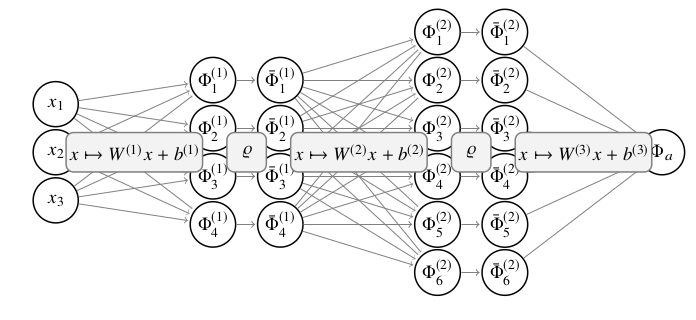
\includegraphics[width=0.5\linewidth]{img/ejemplo_red.png}
\caption{Grafo de una red completamente conectada simple de arquitectura \(a=((3,4,6,1),\mathcal{q})\) donde el primer elemento describe el número de neuronas por capa y el segundo la función de activación. Obtenida en Grohs et al.\cite{matesModernasDL}}.
\label{fig:img1}
\end{figure}


Tras dar una primera aproximación a las redes neuronales completamente conectadas, se comenta que el término redes neuronales profundas hará siempre referencia a esta definición.

Como ya se mencionó anteriormente, las redes neuronales profundas son algoritmos usados en tareas como la clasificación o la regresión que, a partir de cierto subconjunto (de entrenamiento) de un espacio medible, generaliza a datos de otros subconjuntos disjuntos al usado en el entrenamiento. Esto lleva a pensar que, como todo problema en inteligencia artifical, en función de la situación es conveniente usar o no ciertas características determinantes para resolver el problema: la profundidad, las funciones de activación, el número de neuronas por capas,$\dots$. Además, se busca que generalice bien y no sea solo capaz de hacer bien las tareas del conjunto de entrenamiento (sobreajuste), aún queriendo minimizar la función de coste. Estas ideas llevan a pensar en cierto conjunto de posibles algoritmos obtenidos a partir de la arquitectura de una red.

\begin{definicion} [Conjunto de hipótesis de redes neuronales]
Sea $a=(N,\mathcal{q})$ una arquitectura de red neuronal con dimensión de datos de entrada $N_0 = d \in \mathbb{N}$ y de salida $N_L=1$, donde $\mathcal{q}$ es la función de activación (medible). El conjunto de hipótesis de redes neuronales se define de dos maneras en función del tipo de problema:
\begin{itemize}
	\item \textbf{Problema de regresión}: $$\mathcal{F}_a = \{\phi_a(\text{·},\theta): \theta \in \mathbb{R}^{P(N)}\}$$
	\item \textbf{Problema de clasificación}: Con $sgn$ la función signo $$\mathcal{F}_{a,sgn} = \{sgn(\phi_a(\text{·},\theta)):\theta \in \mathbb{R}^{P(N)}\}$$
\end{itemize}
\end{definicion}

Se podría pensar con la definición anterior que basta con ajustar ciertas características de la red para obtener un buen algoritmo que permita generalizar no solo la forma en que los datos entran para ser clasificados, sino también el problema al que estamos enfrentando, siempre que se tenga claro si va a ser de regresión o de clasificación. Esta idea es errónea, tal y como se probará con el siguiente teorema, previas definiciones y resultados para poder construirlo adecuadamente. Gracias a este resultado se podrá entender más adelante porqué no existen algoritmos de ataque o defensa genéricos para cualquier red.

En primer lugar, volviendo a la primera definición dada en el capítulo, se escribe $s=(z^{(i)})_{i=1}^{m}$ a los $m$ datos de un subconjunto de entrenamiento del espacio medible $\mathcal{Z}$. A partir de ahora, se consideran las variables aleatorias e idénticamente distribuidas $Z^{(1)},\cdots,Z^{(m)}$ de cierto vector aleatorio $Z$, cuyas realizaciones se corresponden a los datos $z^{(1)},\cdots,z^{(m)}$ respectivamente, se podría escibir como $z$. Por otro lado, se menciona que $Z$ va a seguir una distribución dada por $I_Z$ en el espacio $\mathcal{Z}$.

\begin{definicion} [Riesgo]

Para toda función $f \in \mathcal{M(X,Y)}$ se define el riesgo como $$\mathcal{R}(f):=\mathbb{E}[\mathcal{L}(f,Z)] = \int_{\mathcal{Z}}\mathcal{L}(f,z) dI_Z(z)$$

Se define también el riesgo para cierta función condicionada a $S$ (vector de variables aleatorias independientes e idénticamente distribuidas, con $f_S=\mathcal{A}(S)$ el modelo asociado a la condicionada), como  
$$\mathcal{R}(f_S)=\mathbb{E}[\mathcal{L}(f_S,Z)|S]$$

\end{definicion}

En líneas generales, se puede observar que el riesgo es ximplemente esperanza matemática de la función asociada al algoritmo.

Para las tareas de predicción se podría escribir $Z = (X,Y)$, esto es, los datos que entran y las respectivas predicciones, por ser $X$ una variable aleatoria que toma valores en $\mathcal{X}$ e Y la respectiva en $\mathcal{Y}$. En los problemas de clasificación, la probabilidad de no predecir bien es

$$\mathcal{R}(f) = \mathbb{E} \left[ \mathbb{1}_{(-\infty,0)} (Yf(X)) \right]$$ 

Además, para datos con ruido es conveniente hacer la siguiente definición.

\begin{definicion} [Función óptima de Bayes]

Teniendo en cuenta la definición anterior, se dirá que $f^{*} \in \mathcal{M(X,Y)}$ es la función óptima de Bayes si minimiza la esperanza, esto es, su riesgo asociado es

$$\mathcal{R}^{*}:= \inf_{f \in \mathcal{M(X,Y)}} \mathcal{R}(f)$$

Nótese que sería incorrecto decir que $\mathcal{R}^{*}=\mathcal{R}(f^{*})$ pues el conjunto $\mathcal{M(X,Y)}$ no es necesariamente compacto, luego puede no alcanzar el mínimo.

\end{definicion}

Los problemas que ocupan a las redes neuronales son los de regresión y clasificación en general, por lo que se puede obtener el riesgo asociado a cada uno de ellos de manera explícita.

\begin{lema}
Considérense $X$ e $Y$ variables aleatorias. El riesgo toma las siguientes expresiones si:
\begin{itemize}
	\item \textbf{Regresión}: Supuesto que $Var[Y] < \infty$, entonces
$$\mathcal{R}(f)=\mathbb{E}[(f(X)-\mathbb{E}[Y|X])^{2}] + \mathcal{R}^{*}$$
alcanzando el mínimo en $f^{*}(x)=\mathbb{E}[Y|X=x]$ para cierto $x \in X \subset \mathcal{X}$.
	\item \textbf{Clasificación}: La expresión viene dada por 
	$$\mathcal{R}(f) = \mathbb{E}[ \left| \mathbb{E}[Y|X] \right| \mathbb{1}_{(-\infty,0)}\left(\mathbb{E}[Y|X]f(X)\right) ] + \mathcal{R}^{*}$$ que alcanza el mínimo en $f^{*}(x)=sgn(\mathbb{E}[Y|X=x])$ para cierto $x \in X \subset \mathcal{X}$.
\end{itemize}
\end{lema}

\begin{lema}\label{lemaNFL}
Sea $\{a_n\}$ una sucesión de números positivos convergente a $0$, tal que $a_1 \leq \frac{1}{16}$. Entonces, se puede encontrar una distribución de probabilidad tal que sus valores $(p_1, p_2, \ldots)$ cumplen $p_1 \geq p_2 \geq \cdots$, y dado $n \in \mathbb{N}$ es cierto que
$$\sum_{i=n+1}^{\infty} p_i \geq \max(8a_n, 32np_{n+1}).$$

\end{lema}

\begin{proof}
Basta encontrar una forma de caracterizar $p_i$ de tal manera que se cumpla

$$\sum_{i=n+1}^{\infty}p_i \geq \max(8a_n,32np_n)$$

Sean los naturales $u < v$, se define $H(v,u)=\sum_{i=u}^{v-1} \frac{1}{i}$. Puede ser encontrada una sucesión de naturales $1=n_1 < n_2 < \dots$ tales que cumplen:
\begin{itemize}
	\item $H(n_{k+1},n_k)$ es creciente.
	\item $H(n_2,n_1) \geq 32$.
	\item $8a_{n_k} \leq \frac{1}{2^k}$ para $k \geq 1$.
\end{itemize}

Para que lo anterior sea cierto, sobre todo la tercera afirmación, se necesita la hipótesis de $a_1 \leq \frac{1}{16}$. Ahora, se define la sucesión $\{c_k\}_{k \in \mathbb{N}}$ como 
$$c_k = \frac{32}{2^kH(n_{k+1},n_k)} \text{ para todo } k \geq 1$$
que es decreciente y resolviendo una serie geométrica se cumple la igualdad 
$$\frac{1}{32}\sum_{k=1}^{\infty} c_kH(n_{k+1},n_k)=\sum_{k=1}^{\infty} \frac{1}{2^k}=1$$

Sea ahora $n \in [n_k,n_{k+1})$, y para dicho natural $p_n = \frac{c_k}{32n}$ con $k \in \mathbb{N}$. Se puede observar que $\{p_n\}$ decrece y

$$\sum_{n=1}^\infty p_n = \sum_{k=1}^{\infty} \frac{c_k}{32} H(n_{k+1},n_k) = 1$$

Finalmente, para todo $n \in [n_k,n_{k+1}),$

\[
\sum_{i=n+1}^{\infty} p_i \geq \sum_{j=k+1}^{\infty} \frac{c_j}{32}H(n_{j+1},n_j) = \sum_{j=k+1}^{\infty} \frac{1}{2^j} = \frac{1}{2^k}
\]

Por la monotonía de $H(n_{k+1},n_k)$, es cierto que $\frac{1}{2^k} \geq c_k = 32np_n$. Por otro lado, $\frac{1}{2^k} \geq 8a_{n_k} \geq 8a_n$, por lo que queda probado el lema.

\end{proof}

Finalmente, se prueba que no existe un algoritmo universal para los problemas que enfrentan las redes neuronales profundas suponiendo distribuciones cualesquiera.

\begin{teorema}[No Free Lunch]

Sea $\{a_n\}_{n \in \mathbb{N}}$ una sucesión de números reales positivos convergente a cero, tal que $a_1 \leq \frac{1}{16}$. Para cualquier algoritmo de aprendizaje para una tarea de clasificación específica $\mathcal{A}$, existe una distribución $I_Z$ desprendida de la distribución $(X,Y)$ tal que, dado $n \in \mathbb{N}$ y cierto conjunto de entrenamiento $S \sim I_Z^n$, se cumple lo siguiente:

$$\mathbb{E}[\mathcal{R}(\mathcal{A}(S))] \geq \mathcal{R}^{*}+a_n$$

\end{teorema}

Antes de comenzar la prueba tal y como se ve en Devroye et al.~\cite{demoNFL} se especifica que un algoritmo de aprendizaje $\mathcal{A}$ es en realidad una secuencia de instrucciones $\{f_n\}$ tal que el error asociado a cada una de ellas para el problema de clasificación, converge a $\mathcal{R}(f^*)$. Por ello, es necesario introducir la siguiente definición.

\begin{definicion}
Las reglas de clasificación serán consistentes para cierta distribución si la sucesión de riesgos esperados converge al menor error, esto es
$$\lim_{n \to \infty} \mathcal{R}(f_n) = \mathcal{R}(f^*)=\mathcal{R}^*$$.
Además, serán fuertemente consistentes si 

$$\mathbb{P}[\lim_{n \to \infty} \mathcal{R}_n = \mathcal{R}^*] = 1$$
\end{definicion}

Este teorema se puede reescribir de la siguiente manera, que será probada.

Sea $\{a_n\}$ una sucesión de positivos convergente a $0$ tal que $a_1 \leq \frac{1}{16}$. Para cada regla, existe una distribución existe una distribución con riesgo nulo tal que 

$$\mathbb{E}[L_n] \geq a_n$$

para todo $n \in \mathbb{N}$ y $L_n$ el error de la probabilidad condicionada según el algoritmo.

\begin{proof}

Consideremos $b=0.b_1b_2b_3\ldots \in [0,1]$ y $B$ una variable aleatoria uniformemente distribuida en $[0,1]$ que escribimos como $B=0.B_1B_2B_3\ldots$. Consideremos ahora la variable aleatoria $X$ tal que cumpla 
$$\mathbb{P}[X=i]=p_i$$
donde $p_i \geq p_{i+1} > 0$ $i\geq 1$ y $\sum_{i=n+1}^{\infty} p_i \geq \max(8a_n,32np_{n+1})$ para $n \in \mathbb{N}$. Nótese que $\{p_n\}_{n \in \mathbb{N}}$ es una sucesión que verifica el lema \ref{lemaNFL}. Sea ahora $Y=b_X$, función dependiente de $X$,  que tiene riesgo asociado $0$. En función de $b \in [0,1)$ va a describir distribuciones distintas, obteniendo una distribución aleatoria si se sustituye por $B$. Escribimos $\Delta_n = ((X_1,B_{X_1}),\ldots,(X_n,B_{X_n}))$ y se define $G_{ni} = f_n(i,\Delta_n)$. Si $L_n(B)$ es la probabilidad de error en un distribución aleatoria, se puede expresar como
$$L_n(B)=\sum_{i=1}^{\infty} p_iI_{\{G_{ni} \neq B_i\}}$$

y si $L_n(b)$ es la probabilidad del error en una distribución parametrizada por $b$, entonces se cumple que

$$\sup_{b} \inf_{n} \mathbb{E} \left[ \frac{L_b(b)}{2a_n} \right] \geq \sup_{b}\mathbb{E}\left[\inf_{n}\frac{L_n(b)}{2a_n}\right] \geq \mathbb{E}\left[\inf_{n}\frac{L_n(B)}{2a_n}\right] = \mathbb{E}\left[\mathbb{E}\left[\inf_{n}\frac{L_n(B)}{2a_n} \bigg| X_1,X_2,\ldots\right]\right]$$

Por otro lado, es cierto que

\begin{align*}
\mathbb{E}\left[ \inf_{n}\frac{L_n(B)}{2a_n} \bigg| X_1,X_2,\ldots \right] &\geq \mathbb{P} \left[ \bigcap_{n=1}^{\infty} \{L_n(B) \geq 2a_n\} \bigg| X_1,X_2,\ldots \right] \\
&\geq 1 - \sum_{n=1}^{\infty} \mathbb{P}\left[ L_n(B) < 2a_n \bigg| X_1,X_2,\cdots \right] \\
&= 1 - \sum_{n=1}^{\infty} \mathbb{P}\left[ L_n(B) < 2a_n \bigg| X_1,_2,\ldots, X_n \right] \\
&= 1 - \sum_{n=1}^{\infty} \mathbb{E} \left[ \mathbb{P} \left[ L_n(B) < 2a_n \bigg| \Delta_n \right] \bigg| X_1,X_2,\ldots,X_n \right]
\end{align*}

A continuación, se usa el concepto de dominancia estocástica por la hipótesis de que $\{p_n\}_{n \in \mathbb{N}}$ es decreciente

\begin{align*}
\mathbb{P}\left[ L_n(B) < 2a_n \,|\, \Delta_n \right] &\leq \mathbb{P} \left[ \sum_{i \notin \{X_1,\ldots,X_n\}} p_i I_{(G_{ni} \neq B_i)} < 2a_n \bigg| \Delta_n \right] \\
&= \mathbb{P}\left[ \sum_{i \notin \{X_1,\ldots,X_n\}} p_iI_{\{B_i=1\}} < 2a_n \bigg| \Delta_n \right] \leq \mathbb{P}\left[ \sum_{i=n+1}^{\infty}  p_iI_{\{B_i=1\}} < 2a_n \right] \\ &= \mathbb{P}\left[ \sum_{i=n+1}^{\infty} p_iB_i < 2a_n \right]
\end{align*}

Para concluir la demostración, se tendrá que usar el método de acotación de Chernoff (véase resultados previos), apoyado en la desigualdad de Markov:

\begin{align*}
\mathbb{P}\left[ \sum_{i=n+1}^{\infty} p_iB_i < 2a_n \right] &\leq \mathbb{E}\left[ e^{2sa_n - s\sum_{i=n+1}^{\infty} p_iB_i} \right] \\ 
&= e^{2sa_n}\prod_{i=n+1}^{\infty}\left(\frac{1}{2} + \frac{1}{2}e^{-sp_i}\right) \leq e^{2sa_n}\prod_{i=n+1}^{\infty}\frac{1}{2}\left(2-sp_i+\frac{s^2p_i^2}{2}\right) \\
&\leq \exp\left(2sa_n + \sum_{i=n+1}^{\infty}\left(-\frac{sp_i}{2}+\frac{s^2p_i^2}{4}\right)\right) \text{ (y como } 1-x \leq e^{-x} \text{)} \\
& \leq \exp\left( 2sa_n - \frac{s\Sigma}{2} + \frac{s^2p_{n+1}\Sigma}{4}\right) \text{ (donde } \Sigma = \sum_{i=n+1}^{\infty} p_i  \text{)} \\
&= \exp\left(-\frac{1}{4} \frac{(4a_n - \Sigma)^2}{p_{n+1}\Sigma} \right)
\end{align*}

teniendo en cuenta que $\Sigma > 4a_n $ y tomando $s = \frac{\Sigma - 4a_n}{p_{n+1}\Sigma}$ se sigue que 

\begin{align*}
\exp\left(-\frac{1}{4} \frac{(4a_n - \Sigma)^2}{p_{n+1}\Sigma} \right) \leq \text{exp}\left( -\frac{1}{16} \frac{\Sigma}{p_{n+1}} \right)
\end{align*}
pues además $\Sigma \geq 8a_n$. Como es cierto $\Sigma \geq 32np_{n+1}$ se concluye que

\begin{align*}
\text{exp}\left( -\frac{1}{16} \frac{\Sigma}{p_{n+1}} \right) \leq e^{-2n}
\end{align*}

por lo que

\begin{align*}
\sup_{b}\inf_{n} \mathbb{E} \left[ \frac{L_n(b)}{2a_n} \right] \geq 1 - \sum_{n=1}^{\infty} e^{-2n} = \frac{e^2-2}{e^2-1} > \frac{1}{2}
\end{align*}

Así, existe un $b$ que cumple lo que se quería probar para todo $n \in \mathbb{N}$

\end{proof}

%Para ilustrar un ejemplo en el que el teorema anterior puede ser usado para ver que no existe un algoritmo universal para todos los problemas de clasificación es el siguiente: seleccionado $\mathcal{F}$ el conjunto de hipótesis, sea $f_{\mathcal{F}}^* \in \text{argmin}_{f \in \mathcal{F}} \mathcal{R}(f)$ la mejor aproximación tal que

%\begin{align*}
%\mathcal{R}(f_S)-R^* &= \mathcal{R}(f_S)- \hat{\mathcal{R}}_S(f_S)+\hat{\mathcal{R}}_S(f_S)-\hat{\mathcal{R}}_S(f_\mathcal{F}^*) + \hat{\mathcal{R}}_S(f_\mathcal{F}^*) - \mathcal{R}_S(f_\mathcal{F}^*) + \mathcal{R}_S(f_\mathcal{F}^*) - \mathcal{R}^*
%\end{align*}


%\begin{align*}
% \leq \epsilon^{\text{opt}} + 2\epsilon^{\text{gen}}+\epsilon^{\text{approx}}
%\end{align*}

Es conveniente remarcar la forma en que una red neuronal profunda puede aprender. Tal y como se observa en \ref{fig:img1}, cada capa con neuronas tienen una serie de funciones de activación. La manera de entrenar y transmitir la información entre las neuronas es a través de la técnica backpropagation. Con esta manera el error en la red se propaga tanto adelante como atrás, siendo la forma más común de hacerlo el cálculo de los gradientes, por lo que es fundamental el uso de la regla de la cadena. La regla de la cadena facilita el control de cómo pequeños cambios en los pesos y sesgos de una capa afectan a la función de pérdida final, lo que es esencial para el ajuste adecuado de los parámetros de la red neuronal.

El clásico algoritmo para permitir que la red aprenda es el gradiente estocástico descendente, que se apoya en hiperparámetros tales como la tasa de aprendizaje. La expresión fundamental de este algoritmo es 

$$\Theta^{(k)} = \Theta^{(k-1)} - \frac{\eta_k}{m'}\sum_{z \in S'} \triangledown_\theta\mathcal{L}(\phi_a(\cdot,\Theta^{(k-1)}),z) $$

siendo $\Theta_k$ los pesos en la red en la iteración $k$ y $m' \leq m$ el tamaño de batch escogido $S'$ de un dataset de entrenamiento $S$.

Una pregunta que podría hacerse es cuán rápido aprende la red para un algoritmo basado en gradiente estocástico descendente. El siguiente teorema no solo asegura la convergencia del algoritmo, sino que trata sobre la velocidad de convergencia del mismo.

\begin{teorema}
Se escribe $D^{(k)}=\triangledown r(\Theta^{(k-1)})$ y $r(\theta)=\hat{\mathcal{R}}_s(\phi_a(\cdot,\theta))$. Sean $p,K \in \mathbb{N}$ y $r:B(0,1) \to \mathbb{R}$ con $B(0,1) \subset \mathbb{R}^p$, siendo $r$ diferenciable y convexa. Sea $(\Theta^{(k)})_{k=1}^{K}$ el conjunto de pesos de cada capa con inicialización $\Theta^{(0)}=0$, tasa de aprendizaje $\eta_k=K^{-\frac{1}{2}}$ para $k=\{1,...,K\}$ y las variables aleatorias $(D^{(k)})_{k=1}^{K}$ que se encuentran casi seguro en la bola unidad, esto es, $||D^{(k)}||_2 \leq 1$. Entonces


$$\mathbb{E}[r(\overline{\Theta})] - r(\theta^*) \leq \frac{1}{\sqrt{K}}$$

donde $\overline{\Theta} := \frac{1}{K} \sum_{k=1}^{K} \Theta^{(k)}$ y $\theta^* \in argmin_{\theta \in B(0,1)} r(\theta)$.
\end{teorema}

Generalmente las redes neuronales con 2 capas son aproximadores universales, es decir, suponiendo una función de activación $\mathcal{q}$ la red neuronal puede aproximar cualquier función continua, por muy compleja que sea, sobre un conjunto compacto. Para acabar el apartado, se enuncia y demuestra el siguiente teorema, siendo necesarios algunos resultados del análisis funcional.

\begin{teorema}[Teorema de aproximación universal]
Sean $d \in \mathbb{N}$, $K \subset \mathbb{R}^d$ un compacto, y $\mathcal{q} \in L_{loc}^{\infty}(\mathbb{R})$ una función de activación tal que la adherencia del conjunto de puntos de discontinuidad de la misma es un conjunto de Lebesgue nulo. Considérese

$$\tilde{\mathcal{F}} = \bigcup_{n \in \mathbb{N}} \mathcal{F}_{((d,n,1),\mathcal{q})}$$


el conjunto de realizaciones de una red neuronal de dos capas. Entonces existe cierto subespacio $C(K) \subset cl(\tilde{\mathcal{F}})$ de funciones continuas sobre $K$ si y solo si no existe ningún polinomio $p: \mathbb{R} \to \mathbb{R}$ tal que $p=\mathcal{q}$ casi por doquier ($cl(\tilde{\mathcal{F}}$ es la adherencia de $\tilde{\mathcal{F}}$ se toma con respecto a la topología inducida por la norma $L^{\infty}(K)$).
\end{teorema}

\begin{proof}
Apoyándose en el teorema de Hahn-Banach, se obtiene que el que $\tilde{\mathcal{F}}$ sea denso sobre cierto espacio vectorial real normado $\mathcal{S}$ es equivalente a afirmar que para todos aquellos funcionales no triviales $F \in \mathcal{S}'-\{ 0 \}$ que estén en el espacio dual topológico de $\mathcal{S}$ existen ciertos parámetros $w \in \mathbb{R}^d$, $b \in \mathbb{R}$ tales que cumplen

$$F(\mathcal{q}(\langle w,\cdot \rangle + b)) \neq 0$$

En el caso en que $\mathcal{S} = C(K)$ entonces por el teorema de representación de Riesz-Markov-Kakutani se tiene que $\mathcal{S'}$ es un espacio de medidas de Borel sobre $K$. Por lo tanto el teorema se prueba si $\mathcal{q}$ es discriminatoria, esto es, $\mathcal{q}$ es tal que para una medida de Borel $\mu$, cumple

$$\int_{K} \mathcal{q}(\langle w,x \rangle + b)d\mu(x) = 0$$

para $w \in \mathbb{R}^d$ y $b \in \mathbb{R}$ si $\mu = 0$. Por ejemplo, si fuese una función activadora sigmoide, sería discriminatoria.

Supóngase que $\mathcal{q}$ es discriminatoria para todo $w \in \mathbb{R}^d$, $b \in \mathbb{R}$. Como para $x \in \mathbb{R}^d$ se tiene que $\mathcal{q}(ax+b) \to \mathbb{1}_{(0,\infty)}(x) + \mathcal{q}(b)\mathbb{1}_{\{0\}}(x)$ si $a \to \infty$, por hipótesis y pasando al límite para $c_1,c_2,b \in \mathbb{R}$, $w \in \mathbb{R}^d$, se obtiene

\[
\int_{K} \mathbb{1}_{[c_1,c_2]}(\langle w,x \rangle + b) \, d\mu(x) = 0
\]

Para finalizar, si se representa la exponencial $e^{-2\pi i x}$ como límite de suma de funciones elementales, lleva a deducir que

\[
\int_{K} e^{-2\pi i (\langle w,x\rangle + b)} \, d\mu(x) = 0.
\]

Por lo tanto, al anularse la transformada de Fourier de $\mu$, se concluye que $\mu = 0$.

\end{proof}

Hasta ahora se ha probado para funciones compactas sobre un espacio compacto. Sin embargo, se puede extender a funciones medibles usando el teorema probado como apoyo, el teorema de Lusin y la medida de Lebesgue.

\section{Aprendizaje adversario}

Los algoritmos de aprendizaje profundo, al igual que el resto de tecnologías informáticas, son propensos a recibir ataques para hacerles fallar. Por ello, el interés por el desarrollo de algoritmos más robustos frente a dichos ataques crece cada vez más, sobre todo con el gran impacto que la inteligencia artificial está teniendo en la vida cotidiana de las personas.

\subsection{Ataques adversarios}

Es adecuado tratar este tipo de ataques como un caso aparte a los clásicos ataques a sistemas informáticos (virus, troyanos,...) ya que la forma de actuar o los objetivos pueden ser distintos. Se denominan ataques adversarios.

Los ataques adversarios pueden ser clasificados según la forma en que actua, conocimientos del algoritmo,... Por ejemplo, se podría clasificar de la siguiente manera (seguida en Joseph et al.~\cite{LibroAdvMachL}):
\begin{itemize}
	\item \textbf{Ataques causativos}: Aprovechan las debilidades que presentan los datos de entrenamiento (mala calidad, escasez,...).
	\item \textbf{Ataques exploratorios}: Orientados a llevar al fallo a modelos ya entrenados que estén en fase de test o ya en uso por otros usuarios.
\end{itemize}

Otras formas de clasificar estos ataques puede ser la propuesta en Zhou et al.~\cite{ArtCentralInfo}:
\begin{itemize}
	\item \textbf{Objetivo del atacante}:
	\begin{itemize}
		\item \textbf{Ataques de envenenamiento}: Los atacantes acceden y modifican el dataset de entrenamiento, haciendo que el sistema no dé los resultados esperados.
		\item \textbf{Ataques de evasión}: Dada una red profunda entrenada, sin poder alterar los pesos, el atacante accede y modifica el dataset de test para conducir al algoritmo a fallar.
	\end{itemize}
	\item \textbf{Conocimiento del sistema atacado}: 
	\begin{itemize}
		\item \textbf{Ataques de caja blanca}: El atacante conoce toda o parte de la información que describe al modelo, creando ataques en base a ella.
		\item \textbf{Ataques de caja negra}: El atacante desconoce las características del algoritmo, por lo que los ataques se dirigen a obtener información del sistema.
	\end{itemize}
	\item \textbf{Comportamiento del algoritmo}:
	\begin{itemize}
		\item \textbf{Ataques sin etiqueta}: El propósito del ataque es hacer que el algoritmo falle una predicción, sin importar el resultado.
		\item \textbf{Ataques con etiqueta}: El ataque hará que el algoritmo falle en su predicción, acorde a lo que especifique el atacante.
	\end{itemize}
\end{itemize}

Nótese que la clasificación no es excluyente entre si. Es decir, un ataque puede ser clasificado tanto de envenenamiento como de ataque con etiqueta.

En la Figura \ref{fig:ataques_scheme} se muestra un esquema general en lo que respecta al ataque según objetivo del atacante.

\begin{figure}[!htbp]
    \centering
    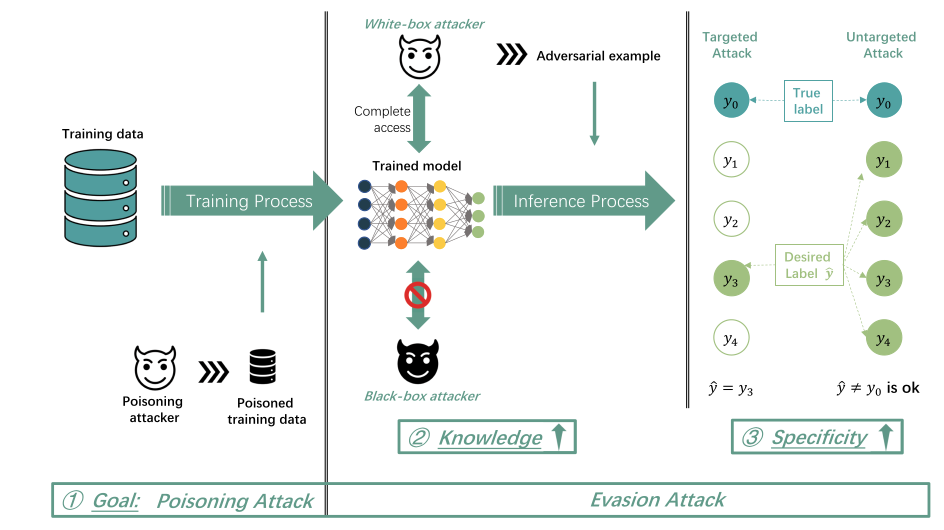
\includegraphics[width=1.0\textwidth]{ataque_objetivo_atacante.png}
    \caption{Imagen que ilustra el esquema general de la forma de atacar a una red neuronal profunda. Obtenida en Rodrigo et al.~\cite{RodrigoTFM}}
    \label{fig:ataques_scheme}
\end{figure}

Si bien es más fácil ver la acción de estos ataques en redes convolucionales para clasificación de imágenes, es posible  adaptar un ataque a cualquier tipo de red, como las redes recurrentes, los modelos LLM, etc. Un ejemplo de ataque a una red convolucional, en que se añade ruido imperceptible al ojo humano, es el que aparece en la Figura \ref{fig:example_fgsm}.

\begin{figure}[h]
    \centering
    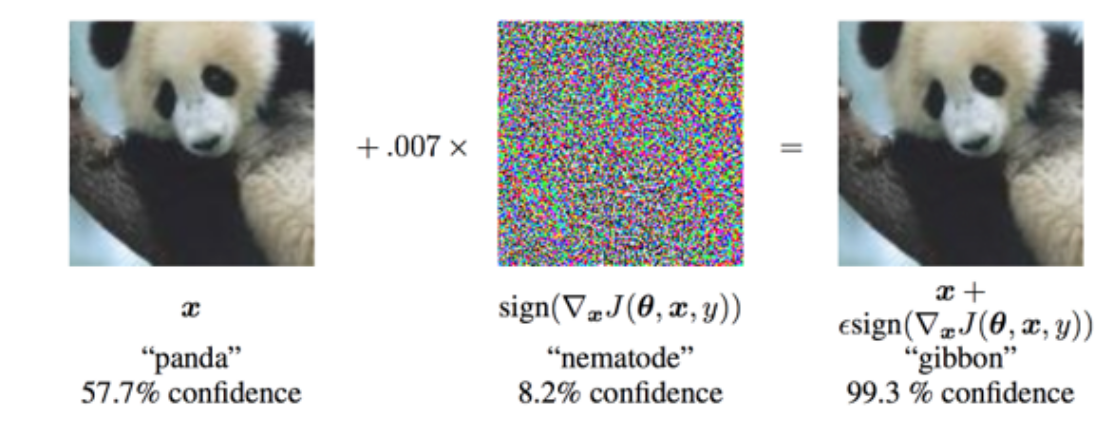
\includegraphics[width=0.7\textwidth]{example_fgsm.png}
    \caption{Ejemplo de ataque FGSM a una red entrenada en Goodfellow et al.~\cite{GoodfLAdvers}}
    \label{fig:example_fgsm}
\end{figure}


La existencia de tales ataques hace pensar en cómo podrían ser evitados, y para ello hay que pensar en qué está fallando en la red para poder ser atacada. Muchos investigadores discuten entre las vulnerabilidades que presentan las redes neuronales, sin llegar a un acuerdo que establezca un paradigma universal de defensa de estos algoritmos.

Por un lado, Ilyas et al.~\cite{NoRobustFeatures} consigue probar que una de las causas es el aprendizaje de características no robustas. Gilmer et al.~\cite{RelatDimensAdvEx} culpa a la alta dimensionalidad de los datos, mientras que otros como Schmidt et al.~\cite{RequiresDataLudwig} estima que se debe a la poca presencia de datos.

También hay otros estudios que buscan las vulnerabilidades al modelo. Por ejemplo, mientras en Szegedy et al.~\cite{DataManifold} culpa a la no linealidad de modelos, otros como Goodfellow et al.~\cite{GoodfLAdvers} y Fawzi et al.~\cite{FundLimits} culpan a la linealidad de los algoritmos, siendo visiones claramente enfrentadas. Además, otros estudios sugieren otras vulnerabilidades como los límites de decisión de la red, o la forma de entrenar a la red.

\subsection{Técnicas de defensa}

Presentada una clasificación de los posibles ataques, y las vulnerabilidades expuestas tanto en los datos como en el propio modelo, es natural intentar idear maneras de entrenar a un algoritmo de aprendizaje profundo para minimizar, o incluso evitar, el daño ocasionado por estos ataques. A continuación se listan algunas técnicas usadas para la mitigación del daño:
\begin{itemize}
	\item \textbf{Robustez de la red}: Mediante el uso de técnicas como la introducción de capas dropout, se podría conseguir que el algoritmo aprendiese características robustas, esto es, identifican al objeto a detectar, pero de una manera más óptima, frente a otras posibles características.
	\item \textbf{Aumento de datos}: La red podría aprender las características que identifican mejor a un objeto de la imagen si el mismo se encuentra en distintas situaciones. Haría que la red generalizase mejor.
	\item \textbf{Detección de datos envenenados}: Aunque muchos datos envenenados serían imposibles de distinguir para un humano, se han desarrollado algoritmos que, dado un dataset, puedan detectar qué datos han sido alterados bajo cierta precisión.
\end{itemize}

\endinput
%--------------------------------------------------------------------
% FIN DEL CAPÍTULO. 
%--------------------------------------------------------------------